%%%------------------------------------------------------------------------------------------------------------
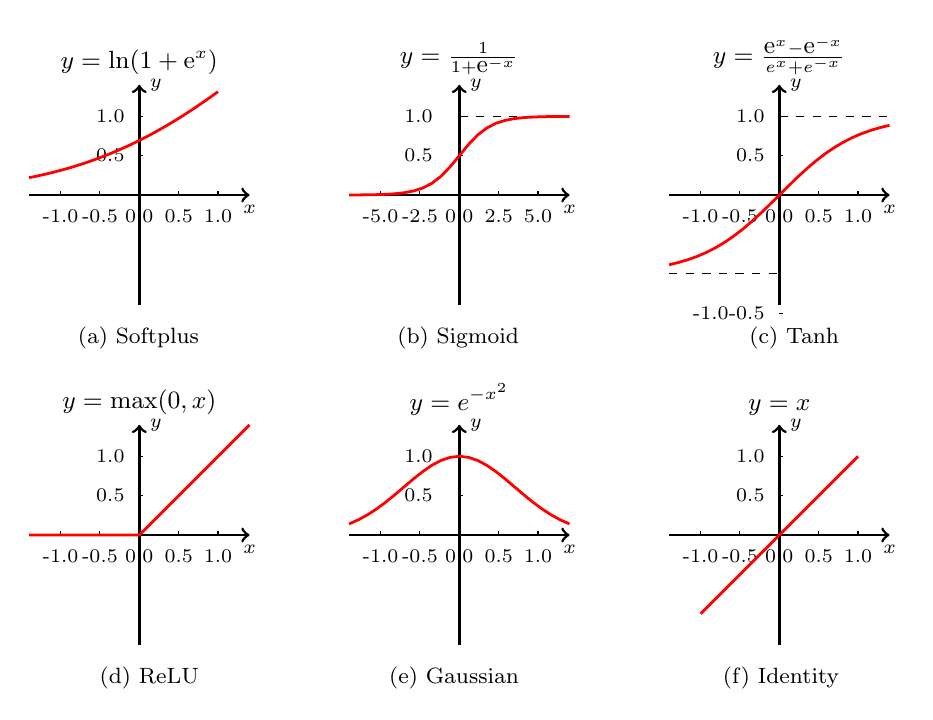
\begin{tikzpicture}
\begin{scope}
\draw[->, line width=1pt](-1.4,0)--(1.4,0)node[left,below,font=\scriptsize]{$x$};
\draw[->, line width=1pt](0,-1.4)--(0,1.4)node[right,font=\scriptsize]{$y$};
\foreach \x in {-1.0,-0.5,0.0,0.5,1.0}{\draw(\x,0)--(\x,0.05)node[below,outer sep=2pt,font=\scriptsize]at(\x,0){\x};}
 \foreach \y in {1.0,0.5}{\draw(0,\y)--(0.05,\y)node[left,outer sep=2pt,font=\scriptsize]at(0,\y){\y};}
\draw[color=red ,domain=-1.4:1, line width=1pt]plot(\x,{ln(1+(exp(\x))});
\node[black,anchor=south] at (0,1.4) {\small $y = \ln(1+{\textrm e}^x)$};
\node [anchor=south east,inner sep=1pt] (labela) at (0.8,-2) {\footnotesize{(a) Softplus}};
\end{scope}

%%%------------------------------------------------------------------------------------------------------------
\begin{scope}[xshift=1.6in]

\draw[->, line width=1pt](-1.4,0)--(1.4,0)node[left,below,font=\scriptsize]{$x$};
\draw[->, line width=1pt](0,-1.4)--(0,1.4)node[right,font=\scriptsize]{$y$};
\draw[dashed](0,1)--(1.4,1);
\foreach \x in {-1,-0.5,0,0.5,1}{\draw(\x,0)--(\x,0.05)node[below,outer sep=2pt,font=\scriptsize]at(\x,0){
      \pgfmathparse{(\x)*5}
      \pgfmathresult};}
\foreach \y in {0.5,1.0}{\draw(0,\y)--(0.05,\y)node[left,outer sep=2pt,font=\scriptsize]at(-0.15,\y){\y};}
\draw[color=red,domain=-1.4:1.4, line width=1pt]plot(\x,{1/(1+(exp(-5*\x)))});
\node[black,anchor=south] at (0,1.4) {\small $y = \frac{1}{1+{\textrm e}^{-x}}$};
\node [anchor=south east,inner sep=1pt] (labelb) at (0.8,-2) {\footnotesize{(b) Sigmoid}};
\end{scope}
%%%------------------------------------------------------------------------------------------------------------

\begin{scope}[xshift=3.2in]
 \draw[->, line width=1pt](-1.4,0)--(1.4,0)node[left,below,font=\scriptsize]{$x$};
        \draw[->, line width=1pt](0,-1.4)--(0,1.4)node[right,font=\scriptsize]{$y$};
        \draw[dashed](0,1)--(1.4,1);
        \draw[dashed](-1.4,-1)--(0,-1);
        \foreach \x in {-1.0,-0.5,0.0,0.5,1.0}{\draw(\x,0)--(\x,0.05)node[below,outer sep=2pt,font=\scriptsize]at(\x,0){\x};}
        \foreach \y in {,-1.0-0.5,0.5,1.0}{\draw(0,\y)--(0.05,\y)node[left,outer sep=2pt,font=\scriptsize]at(0,\y){\y};}
        \draw[color=red ,domain=-1.4:1.4, line width=1pt]plot(\x,{tanh(\x)});
        \node[black,anchor=south] at (0,1.4) {\small $y = \frac{{\textrm e}^{x}-{\textrm e}^{-x}}{{e}^{x}+e^{-x}}$};
\node [anchor=south east,inner sep=1pt] (labelc) at (0.8,-2) {\footnotesize{(c) Tanh}};
\end{scope}

%%%------------------------------------------------------------------------------------------------------------

\begin{scope}[yshift=-1.7in]
  \draw[->, line width=1pt](-1.4,0)--(1.4,0)node[left,below,font=\scriptsize]{$x$};
        \draw[->, line width=1pt](0,-1.4)--(0,1.4)node[right,font=\scriptsize]{$y$};
        \foreach \x in {-1.0,-0.5,0.0,0.5,1.0}{\draw(\x,0)--(\x,0.05)node[below,outer sep=2pt,font=\scriptsize]at(\x,0){\x};}
        \foreach \y in {0.5,1.0}{\draw(0,\y)--(0.05,\y)node[left,outer sep=2pt,font=\scriptsize]at(0,\y){\y};}
        \draw[color=red ,domain=-1.4:1.4, line width=1pt]plot(\x,{max(\x,0)});
        \node[black,anchor=south] at (0,1.4) {\small $y =\max (0, x)$};
\node [anchor=south east,inner sep=1pt] (labeld) at (0.8,-2) {\footnotesize{(d) ReLU}};
\end{scope}

%%%------------------------------------------------------------------------------------------------------------
\begin{scope}[yshift=-1.7in,xshift=1.6in]
        \draw[->, line width=1pt](-1.4,0)--(1.4,0)node[left,below,font=\scriptsize]{$x$};
        \draw[->, line width=1pt](0,-1.4)--(0,1.4)node[right,font=\scriptsize]{$y$};
        \foreach \x in {-1.0,-0.5,0.0,0.5,1.0}{\draw(\x,0)--(\x,0.05)node[below,outer sep=2pt,font=\scriptsize]at(\x,0){\x};}
        \foreach \y in {0.5,1.0}{\draw(0,\y)--(0.05,\y)node[left,outer sep=2pt,font=\scriptsize]at(-0.15,\y){\y};}
        \draw[color=red ,domain=-1.4:1.4, line width=1pt]plot(\x,{exp(-1*((\x)^2))});
        \node[black,anchor=south] at (0,1.4) {\small $y =e^{-x^2}$};
\node [anchor=south east,inner sep=1pt] (labele) at (0.8,-2) {\footnotesize{(e) Gaussian}};
\end{scope}

%%%------------------------------------------------------------------------------------------------------------
\begin{scope}[yshift=-1.7in,xshift=3.2in]
        \draw[->, line width=1pt](-1.4,0)--(1.4,0)node[left,below,font=\scriptsize]{$x$};
        \draw[->, line width=1pt](0,-1.4)--(0,1.4)node[right,font=\scriptsize]{$y$};
        \foreach \x in {-1.0,-0.5,0.0,0.5,1.0}{\draw(\x,0)--(\x,0.05)node[below,outer sep=2pt,font=\scriptsize]at(\x,0){\x};}
        \foreach \y in {0.5,1.0}{\draw(0,\y)--(0.05,\y)node[left,outer sep=2pt,font=\scriptsize]at(0,\y){\y};}
        \draw[color=red ,domain=-1:1, line width=1pt]plot(\x,\x);
        \node[black,anchor=south] at (0,1.4) {\small $y =x$};
\node [anchor=south east,inner sep=1pt] (labelf) at (0.8,-2) {\footnotesize{(f) Identity}};
\end{scope}
\end{tikzpicture}
%%%------------------------------------------------------------------------------------------------------------